\frame{\frametitle{Optimize for BLEU directly}
\begin{center}
\only<1>{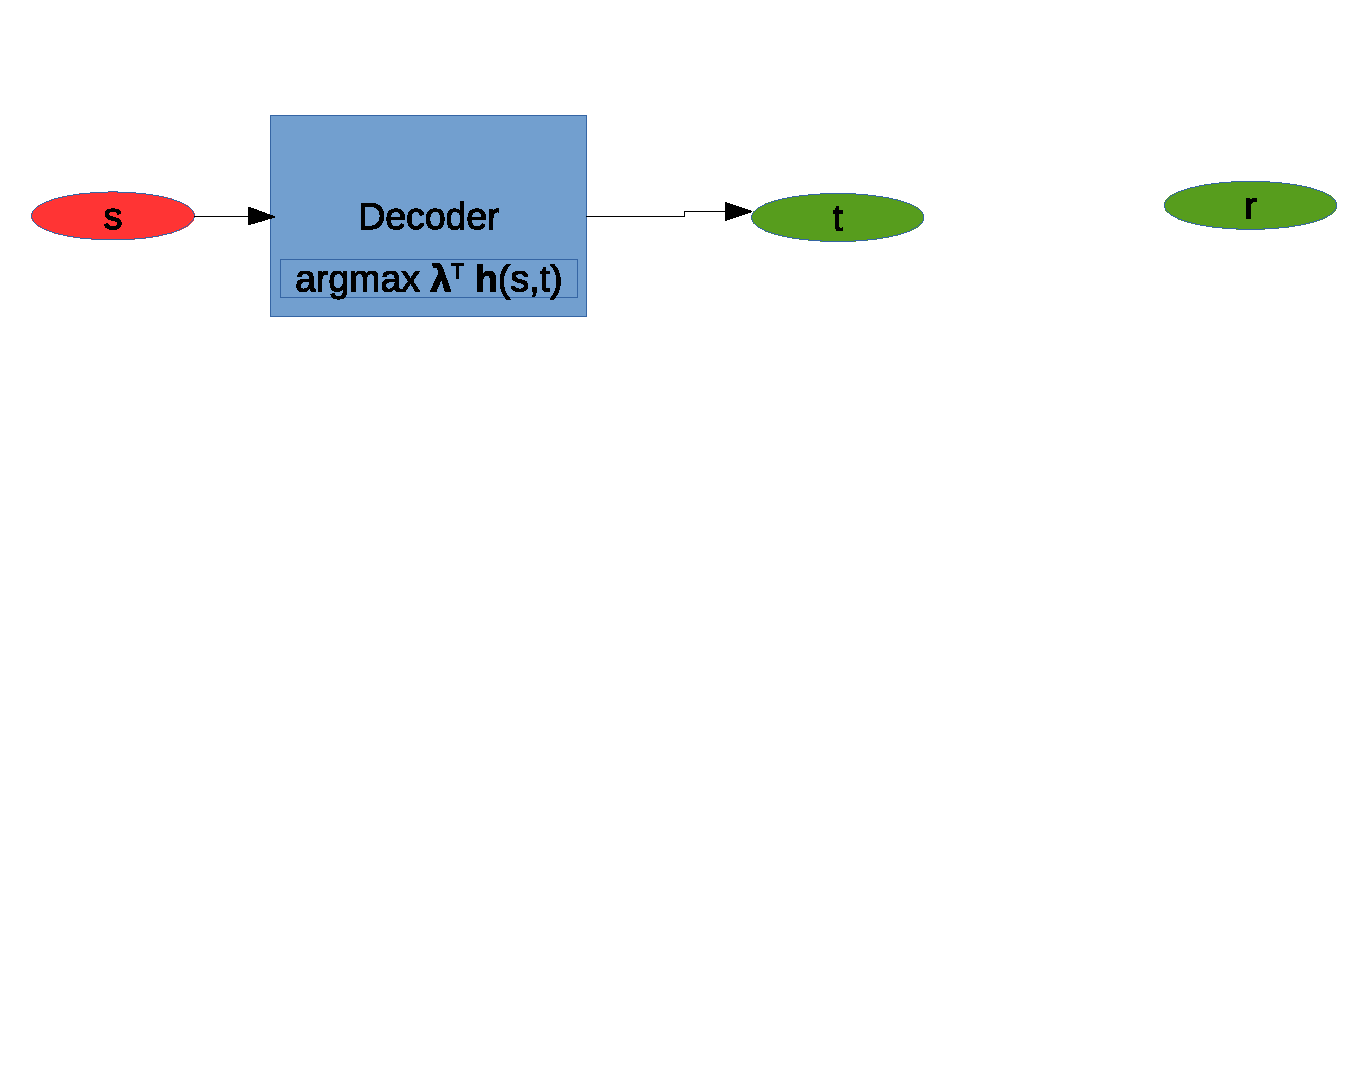
\includegraphics[width=0.70\linewidth]{drawing_discriminative_decoder_tuning1}}
\only<2>{\includegraphics[width=0.70\linewidth]{drawing_discriminative_decoder_tuning2}}
\only<3>{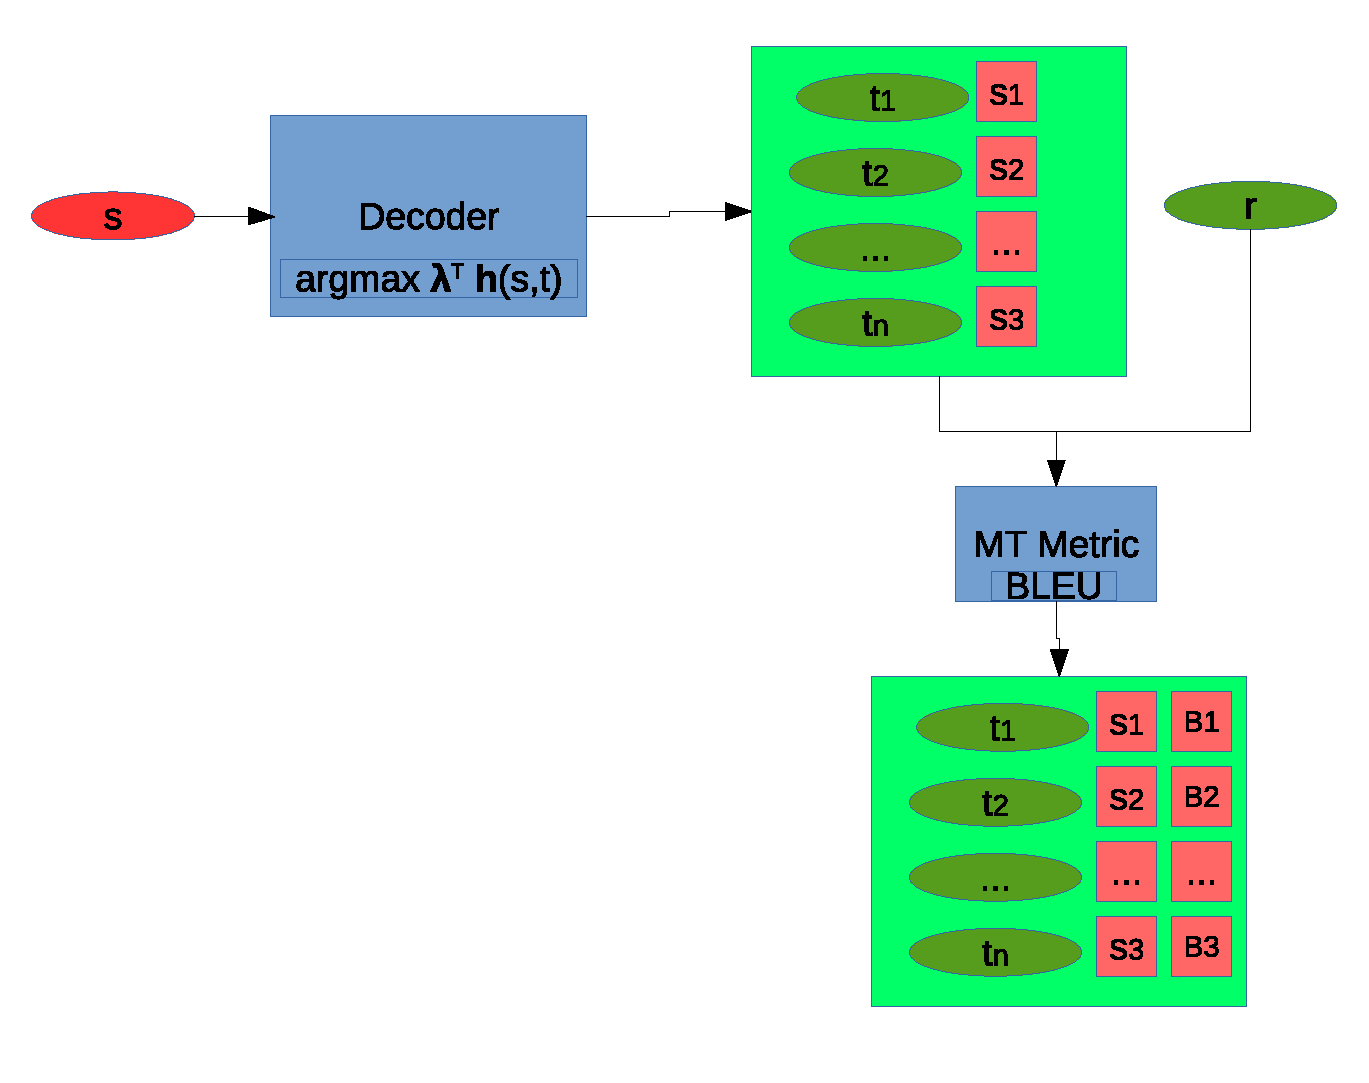
\includegraphics[width=0.70\linewidth]{drawing_discriminative_decoder_tuning3}}
\only<4>{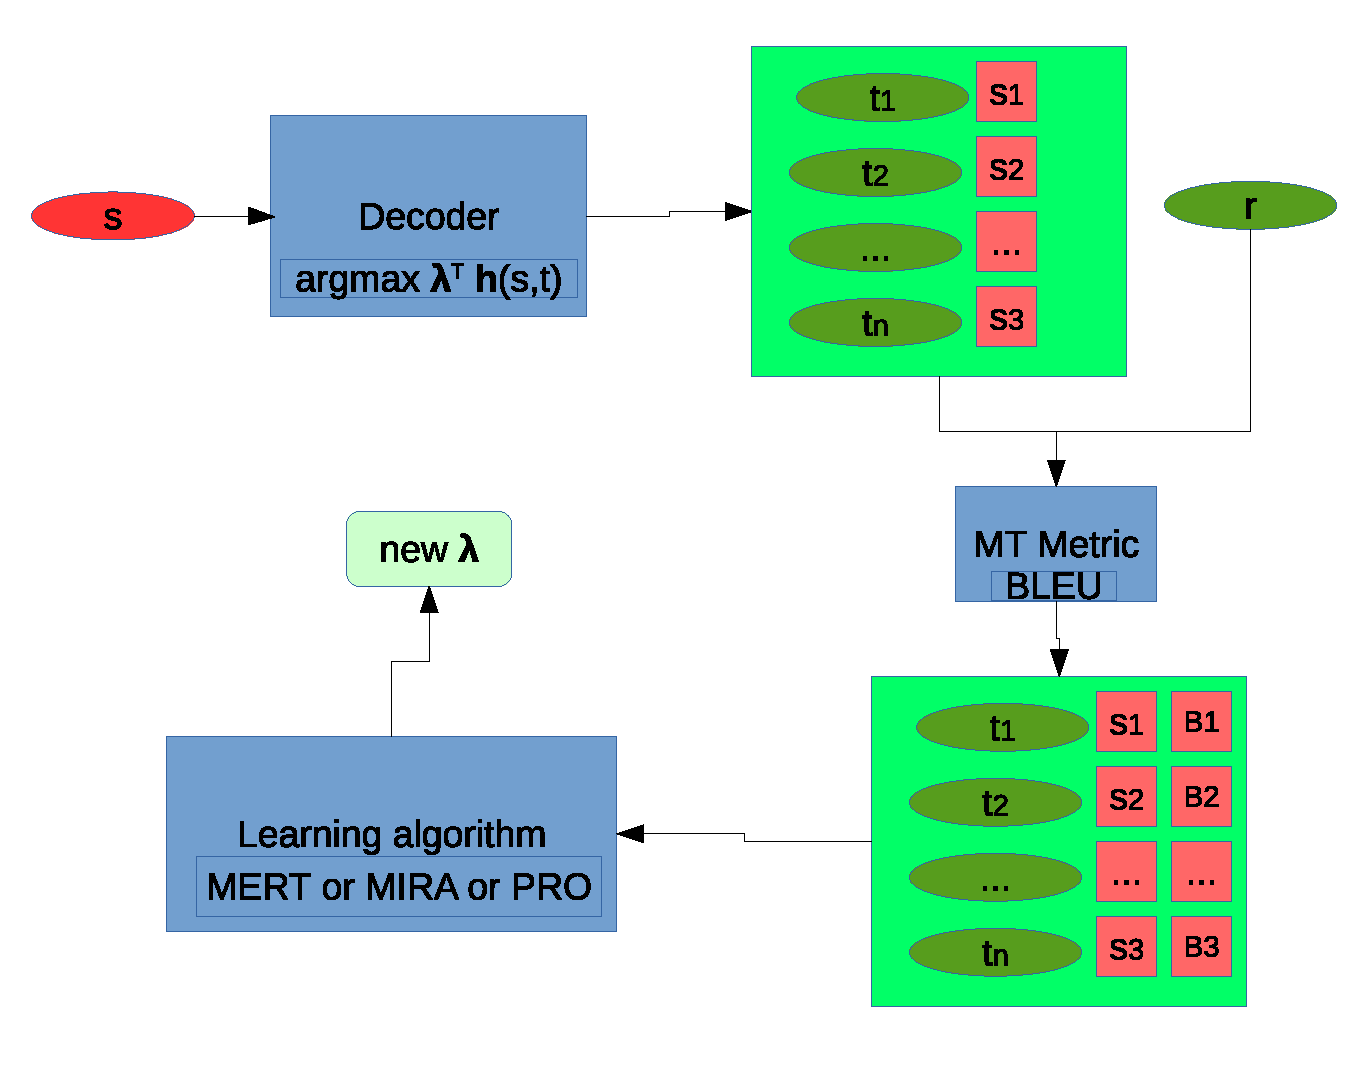
\includegraphics[width=0.70\linewidth]{drawing_discriminative_decoder_tuning4}}
\only<5>{\includegraphics[width=0.70\linewidth]{drawing_discriminative_decoder_tuning5}}
\end{center}

}

\frame{\frametitle{MERT\cite{mert}}
\begin{itemize}
\item MERT is the most often used algorithm for this task
\item Optimizes parameters one by one
\item Directly optimizes objective
\item Works well with systems with small number of features
\end{itemize}
}

\frame{\frametitle{MERT\cite{mert}}
MERT optimizes only one parameter while keeping others fixed.
\begin{align}
\onslide<1->{score(s,t) & = \mathbf{\lambda}^T \mathbf{h}(s,t) \nonumber \\
                        & = \sum_i \lambda_i h_i(s,t)} \nonumber \\
\onslide<2->{& = \lambda_c h_c(s,t) + \sum_{i \neq c}\lambda_i h_i(s,t)} \nonumber \\
\onslide<3->{& = \lambda_c h_c(s,t) + u_c(s,t)} \nonumber
\end{align}

\onslide<4->{\begin{center}
\includegraphics[width=0.60\linewidth]{MERT}
\end{center}}

}

\frame{\frametitle{MERT\cite{mert}}
\begin{center}
\includegraphics[width=0.60\linewidth]{MERT}
\end{center}

\begin{itemize}
\item Extract all \textbf{threshold points} where argmax changes
\pause \item Evaluate each set of threshold points with BLEU score
\pause \item Take the best one and then go again trough the decoding loop
\end{itemize}
}


\frame{\frametitle{MERT\cite{mert}}
\begin{center}
\includegraphics[width=0.60\linewidth]{MERT}
\end{center}

\begin{align}
\onslide<1->{score(s, t_1) & = score(s, t_2) \nonumber}
\onslide<2->{\\ \lambda_c h_c(s,t_1) + u_c(s,t_1) & = \lambda_c h_c(s,t_2) + u_c(s,t_2) \nonumber \\ \nonumber \\ \nonumber}
\end{align}

}

\frame{\frametitle{MERT\cite{mert}}
\begin{center}
\includegraphics[width=0.60\linewidth]{MERT}
\end{center}

\begin{align}
score(s, t_1) & = score(s, t_2) \nonumber \\
\lambda_c \highlight{h_c(s,t_1)} + \highlight{u_c(s,t_1)} & = \lambda_c \highlight{h_c(s,t_2)} + \highlight{u_c(s,t_2)} \nonumber \\
\lambda_c &= \frac{u_c(s,t_1)-u_c(s,t_2)}{h_c(s,t_2)-h_c(s,t_1)} \nonumber
\end{align}

}

\frame{\frametitle{MERT\cite{mert}}
\begin{center}
\includegraphics[width=0.60\linewidth]{MERT}
\end{center}

Few more tricks:
\begin{itemize}
\item We can speed up this by looking for top threshold points\\
start with the steepest line (smallest $h_c(s,t_1)$)\\
$score(x)=\lambda_c \highlight{h_c(s,t_1)} + u_c(s,t_1)$ \\
and find the most negative threshold point for that line
\pause \item Accumulate n-best lists over different decoder runs
\pause \item Average the weights of 3 MERT runs
\end{itemize}
}

\frame{\frametitle{MERT -- good and bad sides}
Good sides:
\begin{itemize}
\item Optimizes corpus level metrics directly.
\end{itemize}

Bad sides:
\begin{itemize}
\item Gets stuck in local minima\\example of finding the highest point in San Francisco \cite{smt_book}
\item Instable: BLEU varies a lot\\
requires at least 3 runs to make it significant \cite{multeval}
\item Cannot handle more than a dozen of features
\end{itemize}
}

